% arara: latexmk: { engine: lualatex, options: [ '-shell-escape' ] }
% arara: latexmk: { clean: 'partial' }
\documentclass[%
  crop,%
  tikz,%
  convert={outext=.svg,command=\unexpanded{pdf2svg \infile\space\outfile}},%
  multi=false%
]{standalone}%
\usepackage[utf8]{luainputenc}%
\usepackage[no-math]{fontspec}%
\defaultfontfeatures{%
  Numbers={OldStyle,Proportional},%
  Ligatures=TeX,%
  Extension=.ttf,%
}%
\setmainfont[%
  UprightFont=*-Regular,%
  ItalicFont=*-Italic,%
  BoldFont=*-Bold,%
  BoldItalicFont=*-BoldItalic,%
]{Raleway}%
\setsansfont[%
  UprightFont=*-Regular,%
  ItalicFont=*-Italic,%
  BoldFont=*-Bold,%
  BoldItalicFont=*-BoldItalic,%
]{Raleway}%
\usepackage[frenchmath]{mathastext}%
\usepackage{amsmath}%
\usepackage{amssymb}%
\usepackage{mathrsfs}%
\usepackage{mathtools}%
\usepackage{siunitx}%
\usepackage[siunitx]{circuitikz}%
\usetikzlibrary{calc,backgrounds,arrows.meta,patterns,positioning}%
\ctikzset{bipoles/length=1.2cm}%

% Colors
\usepackage{xcolor}%
\definecolor{RoseauGreen}{HTML}{cad40e}%
\definecolor{RoseauGrey}{HTML}{adb9cb}%
\definecolor{RoseauBlue}{HTML}{234e83}%

\DeclareMathOperator{\sign}{sign}%

% Sets
\let\C\relax
\newcommand{\R}{\ensuremath{\mathbb{R}}} % Real
\newcommand{\N}{\ensuremath{\mathbb{N}}} % Natural
% \newcommand{\C}{\ensuremath{\mathbb{C}}} % Complexes
\newcommand{\B}{\ensuremath{\mathscr{B}}} % Electrical buses
\newcommand{\Ch}{\ensuremath{\mathscr{C}}} % Loads
\renewcommand{\L}{\ensuremath{\mathscr{L}}} % Lines
\renewcommand{\P}{\ensuremath{\mathscr{P}}} % Phases

% Phases
\newcommand{\arm}{\ensuremath{\mathrm{a}}}%
\newcommand{\brm}{\ensuremath{\mathrm{b}}}%
\newcommand{\crm}{\ensuremath{\mathrm{c}}}%
\newcommand{\nrm}{\ensuremath{\mathrm{n}}}%
\newcommand{\grm}{\ensuremath{\mathrm{g}}}%
\newcommand{\abrm}{\ensuremath{\mathrm{ab}}}%
\newcommand{\bcrm}{\ensuremath{\mathrm{bc}}}%
\newcommand{\carm}{\ensuremath{\mathrm{ca}}}%
\newcommand{\anrm}{\ensuremath{\mathrm{an}}}%
\newcommand{\bnrm}{\ensuremath{\mathrm{bn}}}%
\newcommand{\cnrm}{\ensuremath{\mathrm{cn}}}%
\newcommand{\agrm}{\ensuremath{\mathrm{ag}}}%
\newcommand{\bgrm}{\ensuremath{\mathrm{bg}}}%
\newcommand{\cgrm}{\ensuremath{\mathrm{cg}}}%
\newcommand{\ngrm}{\ensuremath{\mathrm{ng}}}%
\newcommand{\abcrm}{\ensuremath{\mathrm{abc}}}%
\newcommand{\abcnrm}{\ensuremath{\mathrm{abcn}}}%

% Transformer
\newcommand{\Xrm}{\ensuremath{\mathrm{X}}}%
\newcommand{\Yrm}{\ensuremath{\mathrm{Y}}}%
\newcommand{\Zrm}{\ensuremath{\mathrm{Z}}}%
\newcommand{\xrm}{\ensuremath{\mathrm{x}}}%
\newcommand{\yrm}{\ensuremath{\mathrm{y}}}%
\newcommand{\zrm}{\ensuremath{\mathrm{z}}}%
\newcommand{\Arm}{\ensuremath{\mathrm{A}}}%
\newcommand{\Brm}{\ensuremath{\mathrm{B}}}%
\newcommand{\Crm}{\ensuremath{\mathrm{C}}}%
\newcommand{\Nrm}{\ensuremath{\mathrm{N}}}%

% Indices or exponents
\newcommand{\cons}{\ensuremath{\mathrm{cons.}}}%
\renewcommand{\prod}{\ensuremath{\mathrm{prod.}}}%
\newcommand{\theo}{\ensuremath{\mathrm{th.}}}%
\newcommand{\const}{\ensuremath{\mathrm{const.}}}%

% Variables
\newcommand{\umax}{\ensuremath{U^{\max}}}%
\newcommand{\umaxnorm}{\ensuremath{U^{\max\,\text{norm.}}}}%
\newcommand{\umin}{\ensuremath{U^{\min}}}%
\newcommand{\uminnorm}{\ensuremath{U^{\min\,\text{norm.}}}}%
\newcommand{\unom}{\ensuremath{U^{\text{nom.}}}}%
\newcommand{\unomnorm}{\ensuremath{U^{\text{nom.}\,\text{norm.}}}}%
\newcommand{\uup}{\ensuremath{U^{\text{up}}}}%
\newcommand{\uupnorm}{\ensuremath{U^{\text{up}\,\text{norm.}}}}%
\newcommand{\uupprime}{\ensuremath{U^{\text{up}\,\prime}}}%
\newcommand{\udown}{\ensuremath{U^{\text{down}}}}%
\newcommand{\udownnorm}{\ensuremath{U^{\text{down}\,\text{norm.}}}}%
\newcommand{\udownprime}{\ensuremath{U^{\text{down}\,\prime}}}%
\newcommand{\smax}{\ensuremath{S^{\max}}}%
\newcommand{\pmax}{\ensuremath{P^{\max}}}%
\newcommand{\sproj}{\ensuremath{\underline{S^{\text{proj.}}}}}%
%

% UQup = 104.1%, UQmax = 106.3%

\usepackage{pgfplots}%
\pgfplotsset{compat=newest}%
\usepgfplotslibrary{groupplots}%

\begin{document}
  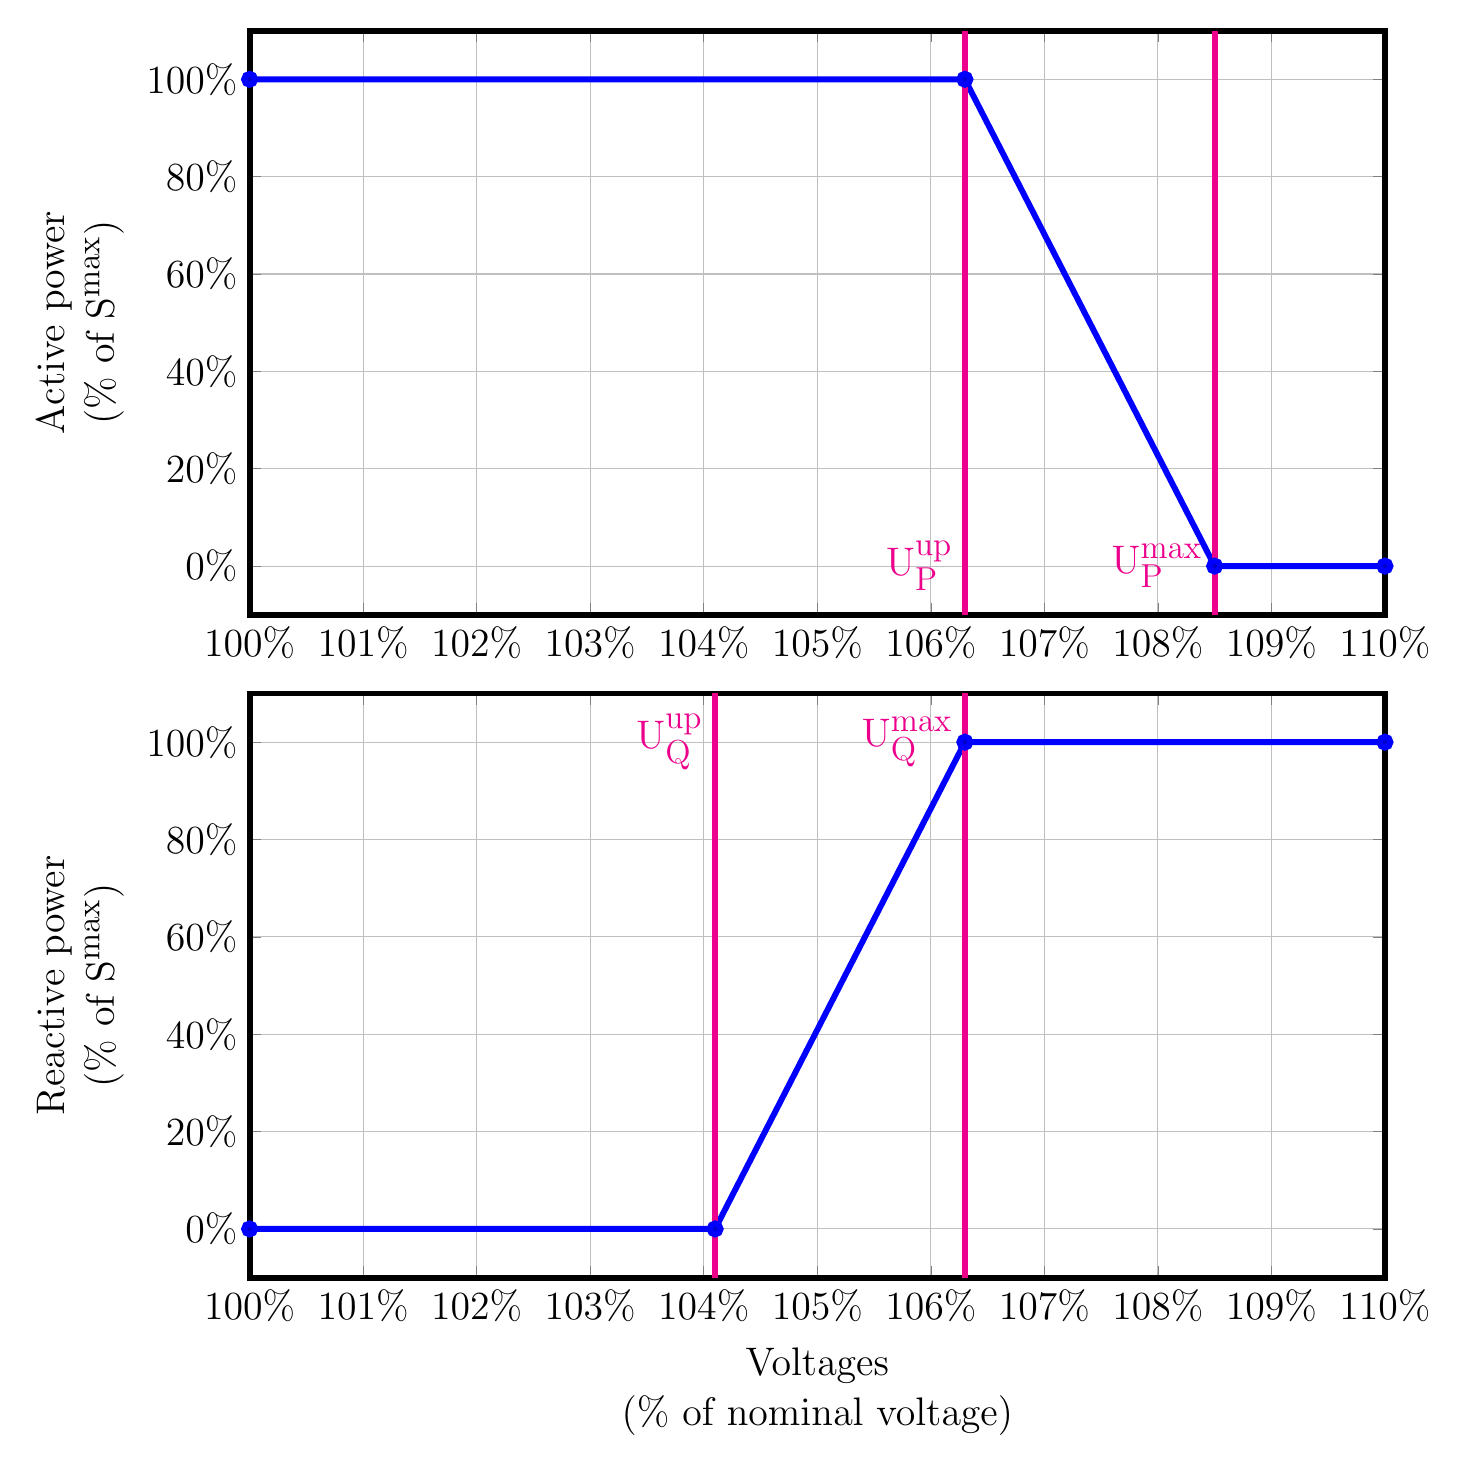
\begin{tikzpicture}[%
    show background rectangle,%
    tight background,%
    background rectangle/.style={fill=white},%
  ]
    \begin{groupplot}
      [%
      group style={group size=1 by 2,
      xlabels at=edge bottom,%
      ylabels at=edge left%
      },%
      xlabel={Voltages\\(\% of nominal voltage)},%
      x label style={at={(axis description cs:0.5,-0.1)},anchor=north, align=center},%
      ylabel={Active power\\(\% of $\smax$)},%
      y label style={at={(axis description cs:-0.1,0.5)},anchor=south, align=center},%
      grid=both,%
      /tikz/line width=0.75mm,%
      /tikz/font={\Large},
%      sharp plot,%
%      mark size=0.5mm,%
      height=9cm,%
      width=16cm,%
      xmin=100,%
      xmax=110,%
      xticklabel style={align=center},%
      xticklabel={%
        $\pgfmathprintnumber{\tick}$\%%
      },%
      yticklabel style={align=center},%
      yticklabel={%
        $\pgfmathprintnumber{\tick}$\%%
      },%
      ]
      \nextgroupplot[ylabel={Active power\\(\% of $\smax$)}]
      \addplot+ coordinates {(100,100) (106.3,100) (108.5,0) (110,0)};%
      \draw[magenta] (axis cs:106.3,\pgfkeysvalueof{/pgfplots/ymin}) -- (axis cs:106.3,\pgfkeysvalueof{/pgfplots/ymax});%
      \draw[magenta] (axis cs:108.5,\pgfkeysvalueof{/pgfplots/ymin}) -- (axis cs:108.5,\pgfkeysvalueof{/pgfplots/ymax});%
      \node[text=magenta, left] at (axis cs:106.3,0) {$U_{\text{P}}^{\text{up}}$};%
      \node[text=magenta, left] at (axis cs:108.5,0) {$U_{\text{P}}^{\max}$};%
      \nextgroupplot[ylabel={Reactive power\\(\% of $\smax$)}]
      \addplot+ coordinates {(100,0) (104.1,0) (106.3,100) (110,100)};%
      \draw[magenta] (axis cs:104.1,\pgfkeysvalueof{/pgfplots/ymin}) -- (axis cs:104.1,\pgfkeysvalueof{/pgfplots/ymax});%
      \draw[magenta] (axis cs:106.3,\pgfkeysvalueof{/pgfplots/ymin}) -- (axis cs:106.3,\pgfkeysvalueof{/pgfplots/ymax});%
      \node[text=magenta, left] at (axis cs:104.1,100) {$U_{\text{Q}}^{\text{up}}$};%
      \node[text=magenta, left] at (axis cs:106.3,100) {$U_{\text{Q}}^{\max}$};%
    \end{groupplot}
  \end{tikzpicture}
\end{document}
% Local Variables:
% mode: latex
% TeX-engine: luatex
% TeX-source-correlate-method-active: synctex
% ispell-local-dictionary: "british"
% coding: utf-8
% LaTeX-indent-level: 2
% fill-column: 120
% End:
